\documentclass[hyperref,utf8]{ctexart}
\usepackage{graphicx}
\usepackage{float}
\usepackage{ragged2e}
\usepackage{amsthm}
\usepackage{amssymb}
\usepackage{amsmath}
\usepackage{wrapfig}
\usepackage{hyperref}
\usepackage[all]{hypcap}
\hypersetup{hypertex=true,
            colorlinks=true,
            linkcolor=red,
            anchorcolor=blue,
            citecolor=red}
\newcommand{\e}{\boldsymbol{\varepsilon}}
\title{笔记}
\author{limbo137}
\date{}

\begin{document}
\maketitle
\section{洛伦兹群的Lie代数}
设
\[{\boldsymbol{\varepsilon}}= 
\begin{bmatrix}
0 & 1 \\ 1 & 0
\end{bmatrix} \]
则
\[x+\varepsilon y=
\begin{bmatrix}
x & y \\ y & x
\end{bmatrix} \]
定义模方:
\[|x+{\boldsymbol{\varepsilon}} y|^2=(x+{\e } y)(x-{\boldsymbol{\varepsilon}} y)=x^2-y^2\]
有
\[e^{{\boldsymbol{\varepsilon}}\lambda}=\cosh{\lambda}+{\boldsymbol{\varepsilon}}\sinh{\lambda}=\begin{bmatrix}
\cosh{\lambda} & \sinh{\lambda} \\ \sinh{\lambda} & \cosh{\lambda}
\end{bmatrix} \]
不难验证$e^{\varepsilon\lambda}$是$O(1,1)$的群元

对于一维体系,发生在$(x,t)$的事件可用$x+{\boldsymbol{\varepsilon}} ct$来表示,则洛伦兹变换(boost)表示为
\[\Lambda=\begin{bmatrix}
\gamma & -\beta\gamma \\ -\beta\gamma & \gamma
\end{bmatrix}=\gamma-{\boldsymbol{\varepsilon}}\beta\gamma\]
对于一个事件$(x,t)$,用洛伦兹变换成$(x',t')$,有
\begin{equation*}
    \begin{split}
        x'+{\boldsymbol{\varepsilon}} ct'
        &=\Lambda(x+{\boldsymbol{\varepsilon}}ct)=(\gamma-{\boldsymbol{\varepsilon}}\beta\gamma)(x+{\boldsymbol{\varepsilon}} ct)\\&=\gamma(x-\beta ct)+{\boldsymbol{\varepsilon}}\gamma(ct-\beta x)
    \end{split}
\end{equation*}
故有洛伦兹变换:
\begin{equation*}
    \begin{split}
    x'&=\gamma(x-\beta ct)\\
    ct'&=\gamma(ct-\beta x)
    \end{split}
\end{equation*}
存在一个$\lambda$,使得一个参考系的洛伦兹变换可表为
\[e^{{-\boldsymbol{\varepsilon}}\lambda}=\gamma-{\boldsymbol{\varepsilon}}\beta\gamma\]
则称这个$\lambda$为该参考系的快度
\section{一维运动}
\subsection{一维匀加速运动}
在固有参考系中,固有时$\tau$定义为\footnote{可见在洛伦兹变换中$\mathrm{d}\tau$是不变的}
\[c\mathrm{d}\tau=\sqrt{c^2\mathrm{d}t^2-\mathrm{d}x^2-\mathrm{d}y^2-\mathrm{d}z^2}=\sqrt{1-\frac{v^2}{c^2}}c\mathrm{d}t\]
其中$v$为相对速度,在一维情形下简化成:\[\mathrm{d}\tau=\sqrt{1-\frac{\dot{x}^2}{c^2}}\mathrm{d}t=\sqrt{1-\beta^2}\mathrm{d}t\]
即得
\[\gamma=\frac{\mathrm{d}t}{\mathrm{d}\tau}\]
位矢(即事件)定义为
\[\tilde{r}=x+{\boldsymbol{\varepsilon}}ct\]
则速度矢量定义为\[\tilde{v}=\frac{\mathrm{d}\tilde{r}}{\mathrm{d}\tau}=\gamma(v+{\boldsymbol{\varepsilon}c})=c\gamma(\beta+{\boldsymbol{\varepsilon}})=c{\boldsymbol{\varepsilon}}e^{{\boldsymbol{\varepsilon}}\lambda}\]
其模方:\[|\tilde{v}|^2=\tilde{v}\tilde{v}^*=-c^2\]
对上式求导,有:\[\frac{\mathrm{d}\tilde{v}}{\mathrm{d}\tau}\tilde{v}^*+\frac{\mathrm{d}\tilde{v}}{\mathrm{d}\tau}^*\tilde{v}=0\]
为保证加速度模长在boost下不变,定义加速度矢量为\[\tilde{a}=\frac{\mathrm{d}\tilde{v}}{\mathrm{d}\tau}\]
即得:
\begin{equation}
    \tilde{a}\tilde{v}^*+\tilde{v}\tilde{a}^*=0 \label{eq:cdot}
\end{equation}

对于一维匀加速运动,我们一般认为我们认为下列这个量保持恒定\footnote{此时的4-加速度为\[a \gamma (1+\e \beta )=a e^{\e \lambda }\]}:
\begin{equation}
\frac{\mathrm{d}(\gamma v)}{\mathrm{d}t}=a=\mathrm{constant}\label{eq:cons}
\end{equation}
用快度改写上式:\[\mathrm{d}\sinh{\lambda}=\frac{a}{c}\mathrm{d}t\]
积分,代入初速度为$0$,令$\rho=\frac{c^2}{a}$,有\[ct=\rho \sinh{\lambda}\]
用(\ref{eq:cons})式除以$\beta=\frac{\mathrm{d}x}{c\mathrm{d}t}$,再积分可得:
\[x=\rho(\cosh{\lambda}-1)\]
联立上两式,得到世界线方程:
\[(x+\rho)^2-(ct)^2=\rho^2\]
是双曲线方程
\subsection{一维振动}
对于一个体系,固有时$\tau$与参考系无关,因此力学体系的作用量应该正比于该积分,即
\[S=\alpha\int c\mathrm{d}\tau=\alpha\int\sqrt{1-\frac{v^2}{c^2}}c\mathrm{d}t\]
我们应该保证真实路径该积分最小,对于自由粒子,真实路径的该积分反而最大,另一方面,作用量中应该含有粒子本身的性质——质量,最后,被积函数(即Lagrange量)应该具有能量量纲,于是我们令$\alpha=-mc$则作用量表为:\[S=-\int mc^2\sqrt{1-\frac{v^2}{c^2}}\mathrm{d}t\]
得到Lagrange量:\[L=-mc^2\sqrt{1-\frac{v^2}{c^2}}=-\frac{mc^2}{\gamma}=-\frac{mc^2}{\cosh{\lambda}}\]
对于一维运动,定义动量为\[p=\frac{\mathrm{d}L}{\mathrm{d}v}=-mc\frac{\mathrm{d}\cosh^{-1}{\lambda}}{\mathrm{d}\tanh{\lambda}}=mc\sinh{\lambda}=mc\beta\gamma\]
顺便我们得到能量表达式:\[E=pv-L=mc^2\gamma\]
静止时得到粒子静质能$mc^2$

以上讨论是对于自由粒子而言的,对于具有形如$U(x)=\frac12 kx^2$势能的粒子,Lagrange量为\[L=-mc^2\sqrt{1-\frac{v^2}{c^2}}-\frac12 kx^2\]
代入Lagrange方程$\frac{\mathrm{d}}{\mathrm{d}t}\frac{\mathrm{d}L}{\mathrm{d}v}=\frac{\mathrm{d}L}{\mathrm{d}x}$,可得到运动方程,但是我们不必去解这个方程,我们应该另辟蹊径来寻找一些定性的结论,这个体系是保守的,故有能量守恒(也可通过运动方程积分得到):
\[E=\frac{mc^2}{\sqrt{1-\frac{v^2}{c^2}}}+\frac12 kx^2\]
将此式无量纲化
\[\frac{E}{mc^2}=\frac{1}{\sqrt{1-\frac{v^2}{c^2}}}+ \frac12 (\frac{\omega x}{c})^2\]
以$x$为横坐标,$\frac{v}{c}$为纵坐标,取几个能量的值,作图
\begin{figure}[H]
    \centering
    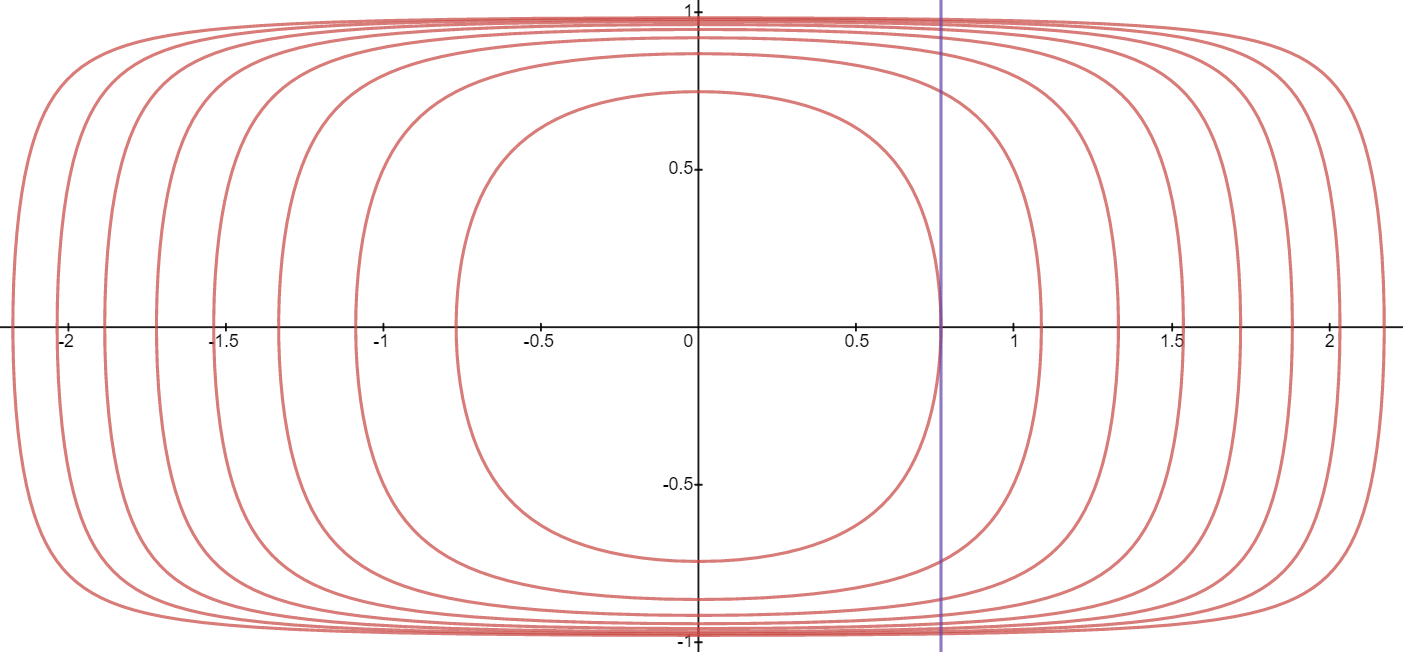
\includegraphics[scale=0.4]{2020-08-26 224653.png}
\end{figure}
靠近中心的红线是能量低的体系,远离的则是高能体系,可以看出,最大速度不会超过$c$,而图中蓝线对应$x=\frac{c}{\omega}$,即振幅的位置
\subsection{一维碰撞}
定义动量矢量:\[\tilde{p}=m\tilde{v}=p+mc\gamma{\boldsymbol{\varepsilon}}\]其模方:\[\tilde{p}\tilde{p}^*=p^2-m^2c^2\gamma^2=-m^2c^2\]
整理得到\[(pc)^2+(mc^2)^2=E^2\]
对于光子等零质量的粒子,有\[E=pc\]顺便得到
自由粒子的Hamilton量:\[H=\sqrt{(pc)^2+(mc^2)^2}\]

两个粒子,质量为$m_1$和$m_2$,速度为$v_1$,$v_2$,在同一直线上,碰后仍在同一直线上,速度为$v'_1$,$v'_2$,有动量守恒:
\begin{equation}
\tilde{p}_1+\tilde{p}_2=\tilde{p}'_1+\tilde{p}'_2
\end{equation}
待定系数:
\begin{equation}
    p_1+p_2=p'_1+p'_2=P\label{eq:4}
\end{equation}
\begin{equation}
m_1\gamma_1+m_2\gamma_2=m_1\gamma'_1+m_2\gamma'_2=\frac{E}{c^2}\label{eq:5}
\end{equation}
我们用两个粒子的$\beta$分别做横纵坐标,画出上两个方程对应的图像
\begin{figure}[H]
    \centering
    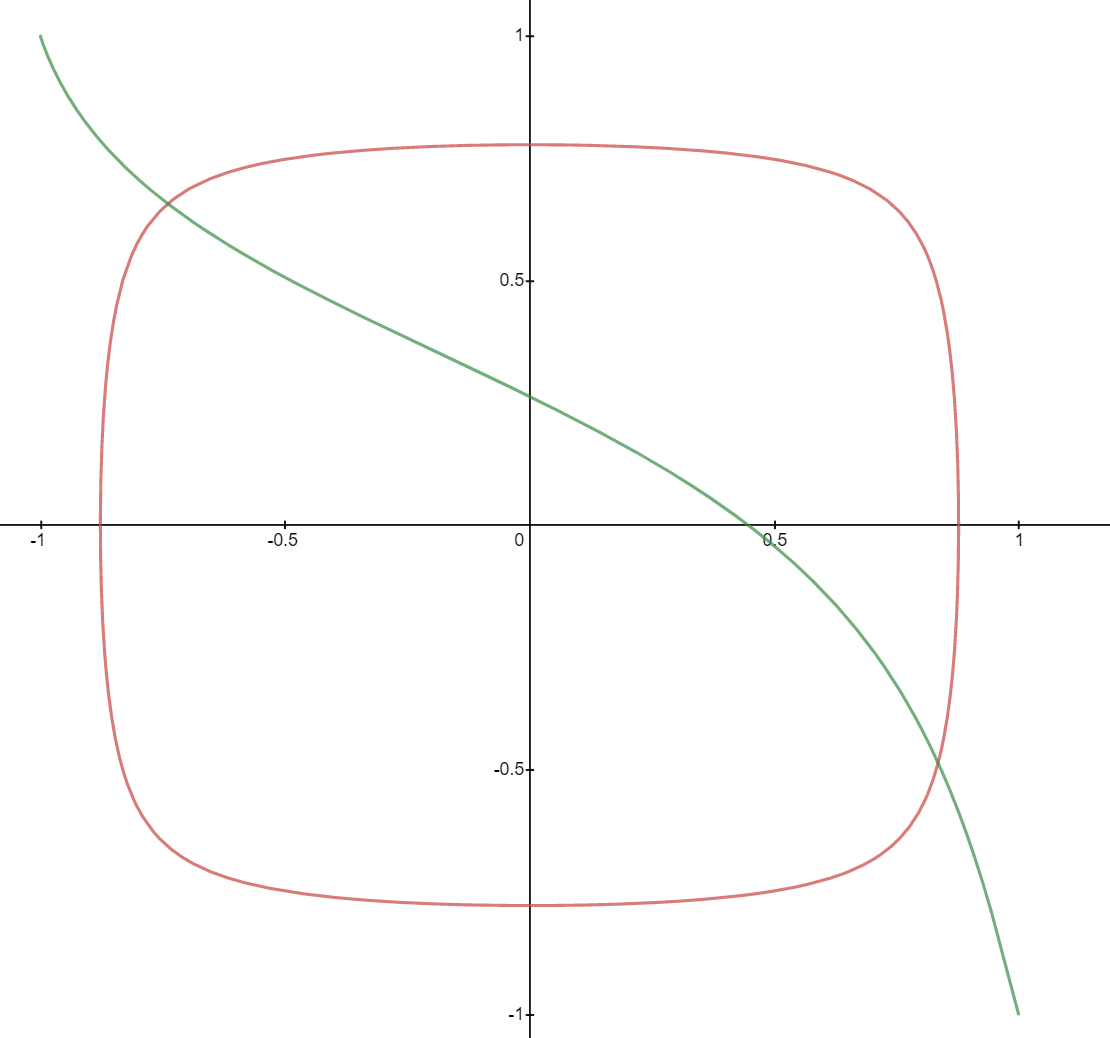
\includegraphics[scale=0.3]{2020-08-27 141243.png}
\end{figure}
绿线代表方程(\ref{eq:4}),红线代表方程(\ref{eq:5}),红绿线一般有两个交点,一个为初态,另一个为末态,我们有几条定性的结论

1.与非相对论情形相同,若$m_1=m_2$,则两粒子速度交换(因为方程完全对称)

2.无论总能量多么高,最大速度不会超过$c$

3.若$m_1<<m_2$,则$v'_1\approx-v_1$,$v'_2\approx v_2$

我们现在来推导柯尼希定理,为方便,我们使用快度,在质心系有:
\[(m_1+m_2)\sinh{\lambda_c}=m_1\sinh{\lambda_1}+m_2\sinh{\lambda_2}\]
得到
\begin{equation*}
    \begin{split}
    \sinh{\lambda_c}&=\frac{m_1\sinh{\lambda_1}+m_2\sinh{\lambda_2}}{m_1+m_2}\\
    \cosh{\lambda_c}&=\sqrt{1+(\frac{m_1\sinh{\lambda_1}+m_2\sinh{\lambda_2}}{m_1+m_2})^2}\\
    &=\frac{\sqrt{(m_1\cosh{\lambda_1}+m_2\cosh{\lambda_2})^2+2m_1m_2(1+\sinh{\lambda_1}\sinh{\lambda_2}-\cosh{\lambda_1}\cosh{\lambda_2})}}{m_1+m_2}\\&=\frac{\sqrt{(m_1\cosh{\lambda_1}+m_2\cosh{\lambda_2})^2+2m_1m_2(1-\cosh{(\lambda_1-\lambda_2)})}}{m_1+m_2}
    \end{split}
\end{equation*}
于是有质心动能表达式:
\[\frac{E_\text{质心}}{c^2}=(m_1+m_2)\cosh{\lambda_c}=\sqrt{(m_1\cosh{\lambda_1}+m_2\cosh{\lambda_2})^2+2m_1m_2(1-\cosh{(\lambda_1-\lambda_2)})}\]
设总能量:
\[E=m_1c^2\cosh{\lambda_1}+m_2c^2\cosh{\lambda_2}\]
于是柯尼希定理写成:
\[E^2=E^2_\text{质心}+2m_1m_2c^4(\gamma_u-1)\]
其中$\gamma_u$定义成
\[\gamma_u=\gamma_1 \gamma_2(1-\frac{v_1 v_2}{c^2})\]
两边开平方,做一些近似:
\[(m_1+m_2)c^2+\frac12 m_1v^2_1+\frac12 m_2cv^2_2=(m_1+m_2)c^2\sqrt{(1+\frac{v^2_c}{2c^2})^2+\frac{m_1m_2}{(m_1+m_2)^2}\frac{u^2}{c^2}}\]
当体系中各速度均远小于光速时,上式可近似为:
\[\frac12 m_1v^2_1+\frac12 m_2v^2_2=\frac12 (m_1+m_2)v^2_c+\frac12 \frac{m_1m_2}{(m_1+m_2)}u^2\]
即经典力学中的柯尼希定理

\section{静力学}
我们定义力矢量
\begin{equation}
    \tilde{f}=m\tilde{a}=\gamma\frac{\mathrm{d}\tilde{p}}{\mathrm{d}t}=\gamma\frac{\mathrm{d}(p+mc\gamma{\boldsymbol{\varepsilon}})}{\mathrm{d}t} \label{eq:force}
\end{equation}
引入空间力$f=\frac{\mathrm{d}p}{\mathrm{d}t}$,则力矢量写成\[\tilde{f}=\gamma(f+{\boldsymbol{\varepsilon}}\frac{\mathrm{d}E}{c\mathrm{d}t})=\gamma(f+{\boldsymbol{\varepsilon}}\frac{P}{c})\]
不过我们想利用(\ref{eq:force})式,利用快度改写,有
\begin{align}
    \tilde{f}&=\cosh \lambda \frac{\mathrm{d}\tilde{p}}{\mathrm{d}t}=\cosh \lambda \frac{\mathrm{d}(p+mc\gamma{\boldsymbol{\varepsilon}})}{\mathrm{d}t} \nonumber \\ 
    &=mc\cosh \lambda\frac{\mathrm{d}(\cosh{\lambda}+\e \sinh{\lambda})}{\mathrm{d}t} \nonumber \\
    &=mc (\cosh^2 \lambda  +\e  \cosh \lambda \sinh \lambda  )\frac{\mathrm{d}\lambda }{\mathrm{d}t}\label{eq:work1}
\end{align}
又因为
\[\frac{\mathrm{d}x}{\mathrm{d}t}=c\tanh \lambda \]
用(\ref{eq:work1})除以上式
\begin{equation}
    \tilde{f}=mc^2\e (\e \cosh \lambda  \sinh \lambda +  \sinh^2 \lambda  )\frac{\mathrm{d}\lambda }{\mathrm{d}x}\label{eq:work2}
\end{equation}
利用(\ref{eq:work1})和(\ref{eq:work2})
\begin{equation*}
    \tilde{f}(c\mathrm{d}t-\e \mathrm{d}x)=mc^2\mathrm{d}\lambda 
\end{equation*}
稍微改写一下
\begin{equation}
    \tilde{f}e^{-\e \lambda }=mc\frac{\mathrm{d}\lambda }{ \mathrm{d}\tau}
\end{equation}
我们还知道
\[\mathrm{d}\tilde{r}^*=-c\e e^{-\e \lambda }\mathrm{d}\tau\]
代入有
\[\tilde{f}\mathrm{d}\tilde{r}^*=-\e mc^2\mathrm{d}\lambda \]
其共轭是
\[\tilde{f}^*\mathrm{d}\tilde{r}=\e mc^2\mathrm{d}\lambda \]
这也印证了(\ref{eq:cdot})式,4-加速和4-速度是互相垂直的,所以上面这个结论虽然形式上类似做功,但却是某种力和位移的外积,还赋予了快度 $\lambda $新意义
\[\Delta \lambda=\frac{1}{\e mc^2}\int^{\tilde{r_2}}_{\tilde{r_1}} \tilde{f}^*\mathrm{d}\tilde{r}\] 
由(\ref{eq:force})我们得出粒子做匀速运动的充要条件为所受的4-力为0
\section{3+1维情形}
受上面的做法启发,我们尝试将4-矢量定义成下面的样子
\begin{equation}
    \tilde{v}=c \gamma(I+\vec{\beta}\cdot\vec{\sigma}) \label{eq:3+1}
\end{equation} 
其中 $\vec{\beta}\cdot\vec{\sigma}$定义成
\[\vec{\beta}\cdot\vec{\sigma}=\beta_{x} \sigma_{x}+\beta_{y} \sigma_{y}+\beta_{z} \sigma_{z}\] 
其中 $\sigma_i$是pauli矩阵,定义成
\[\sigma_x=\begin{pmatrix}
    0&1\\1&0
\end{pmatrix},\sigma_y=\begin{pmatrix}
    0&-i\\i&0
\end{pmatrix},\sigma_z=\begin{pmatrix}
    1&0\\0&-1
\end{pmatrix}\]
可以验证:
\[e^{\lambda\vec{n}\cdot\vec{\sigma}}=(I\cosh \lambda+\vec{n}\cdot\vec{\sigma}\sinh \lambda)\]
所以(\ref{eq:3+1})可以写成
\begin{equation*}
    \tilde{v}=c e^{\lambda \vec{n}\cdot\vec{\sigma}}
\end{equation*}
其中
\[\vec{n}=\frac{\vec{v}}{v}\]
所以洛伦兹变换表示为
\[\Lambda=e^{-\lambda \vec{n}\cdot\vec{\sigma}}\]
下面有一个有用的公式可以帮助计算

\end{document}